\documentclass[]{article}
\usepackage[margin=1in]{geometry}
\usepackage[affil-it]{authblk}
\usepackage{lipsum}
\usepackage{graphicx}
\usepackage{enumitem}
\usepackage{multirow}
\usepackage{natbib}
\usepackage{notoccite}
%\usepackage{gensymb}
\newcommand\litem[1]{\item{}}


%add abstract from Latifa
%use [!htb] for figure placement
%finish reference formatting

%opening
\title{R$\&$D Proposal for EIC Background Studies and the Impact on the IR and Detector design}
\author[1]{Latifa Elouadrhiri
	\thanks{Electronic address: \texttt{latifa@jlab.org}; Latifa Elouadrhiri, Principal Investigator}}
%\author[1]{Yulia Furletova}
\author[2]{Charles Hyde}
%\author[1]{Tim Minkowski}
\author[1]{Vasiliy Morozov}
\author[1]{Kijun Park}
\author[3]{Christine Ploen}
%\author[1]{Marci Stutzman}
\author[4]{Mike Sullivan}



\affil[1]{Thomas Jefferson National Accelerator Facility}
\affil[2]{Old Dominion University}
\affil[3]{University of Connecticut}
\affil[4]{SLAC}

\begin{document}
\date{June 16, 2017}
\maketitle

\begin{abstract}
%first line taken from BNL proposal
In this proposal, we request funding to perform simulations in great detail of the EIC machine related backgrounds and, by quantitative procedure, evaluate the background radiation reaching the experimental detectors. The detectors must be sufficiently well protected to prevent both excessive component occupancies and deterioration from radiation damage. Experience has shown that synchrotron radiation and beam interactions with residual beamline gas are major sources of background that require mitigation. However, other sources must be investigated and their impacts assessed. The type and quantity of background signal impacts the technology choices for the central and auxiliary detectors. There is an effort at Brookhaven National Lab to study beam gas interactions; however, it is primarily focused on the eRHIC design. We propose to independently verify the results of that study and apply the concepts developed at BNL to the JLEIC configuration. Moreover, we would like to advance these studies further by designing a detector beam pipe, considering the impact of the crab crossing, and modeling an extensive section of the accelerator. Thus, this study aims to identify the dominant background sources, quantify their impacts on the detectors and physics, and explore mitigation options as needed. These studies are essential and should be developed alongside the interaction region design, since the backgrounds are dependent on details of the machine lattice and beam optics. Knowledge gained will provide critical information to the machine and detector designs at both JLEIC and eRHIC. Collaboration between the accelerator and physics groups from both laboratories is necessary and will support an iterative design process that maximizes the capabilities of the physics program at an EIC. 



%add hadronic and leptonic background fluctuations due to crab crossing bunch tilt in horizontal plane.

%add development of beam pipe shape which optimizes acceptance and iminizes interaction with beam pipe particles.

%add synchrotron radiation contributions from electron beam interacting with residual beam gas and evaluation of small chicane to minimize this source of background.

% add first look at vacuum system design by determining viability of pump placement options and baseline vacuum level achievable with minimal scheme.

%add checking BNLs results with independent approach (benchmarking their results?)


\end{abstract}

\newpage

\tableofcontents

\newpage

\section{Introduction}

The machine design directly impacts the quantity and type of radiation reaching detectors in the interaction region, which influences the both the physics program and the materials which can be used in the detectors.  Background radiation also greatly affects the systematic uncertainty.  It is important to minimize and fully understand the systematic uncertainty, as it will dominate the high-precision physics measurements at high luminosity.  Specifically, background radiation is influenced by the arrangement of magnet lattice which guides the beam, bunch spacing, beam current, and beam optics, which are being decided now.  Therefore it is critical to perform a thorough study of the type and dose of machine-induced background now, while decisions regarding the interaction region layout are being made.  This insight will enable informed decisions which minimize and mitigate sources of background at the early design phase and to inform detector placement and technology choices as well.  As such, close collaboration between the accelerator and physics divisions will be necessary to inform the design process and maximize the potential of the physics program at the EIC.

Drawing upon the extensive experience of earlier facilities, especially the previous electron-proton collider at HERA at DESY, we are further motivated to perform a detailed study of the backgorund in the IR.  In many ways, the EIC is an extension of the previous collider, which strove to push the limits of luminosity upwards by a factor of seven following the installation and commissioning of the upgrade during 2001/2002.  However, the upgraded machine lattice and beam optics generated severe levels of background in the interaction region.  The primary sources of background were direct synchrotron radiation and beam gas scattering due to vacuum degradation.  After a several-month shutdown, detailed background studies were performed and solutions to mitigate the background were installed.  Ultimately the problems were addressed and the HERA-II upgrade was a success, increasing luminosity by a factor of five; however, this experience underscores the need to complete detailed studies during the design phase as a close collaboration between both physics and accelerator design experts, rather than after the commissioning is complete.  The HERA-II machine shutdown, delays, and post-design changes lend gravitas to our proposed study and strengthens the case for funding.

In summary, we propose a study to determine the quantity, type, and distribution of machine-induced background in the interaction region.  These findings will provide crucial insight to both accelerator and physics divisions, informing choices for interaction region design and detector technology and placement.  Comprehensive knowledge about the radiative environment of the interaction region is essential to guide the current and future design phases.


\section{Background Sources}

Detailed simulations must be performed for relevant background sources.  Sources of background observed at other facilities are listed below, followed by relevant information and its potential impact on detectors.
\begin{itemize}
	\item Synchrotron radiation
	\item Beam-gas interactions
	\item Beam halo
	\item Beam loss
	\item Neutron flux
	\item Radiation from elastic scattering
\end{itemize}

\subsection{Synchrotron radiation}

Synchrotron radiation can significantly impact physics measurements in both main and auxiliary detectors.  It is primarily generated as the electron beam bends through the machine lattice magnets.  In addition to impacting the detector systems, synchrotron radiation can have a deleterious effect on the vacuum quality by heating residual beam gas or causing enhanced desorption of gas from vacuum chamber walls.  This, in turn, causes beam loss due to interactions with the ion beam.  Furthermore, excessive heating due to synchrotron radiation could damage flanges, gaskets, and certain types of detector technology.

Current JLEIC design attempts to reduce the amount of synchrotron radiation generated and lessen its effects on the ion beam and surrounding detectors.  The long, straight section of electron beam line pipe prevents much contribution from the magnet lattice, and the large beam crossing angle mitigates the effect of synchrotron radiation on vacuum quality in the IR. [reference S. Sosa crab X and/or F. Lin MEIC Background 1st look]
%Elke disusses placement of the lumi monitor, need for bgs to provide input to this particular detector.  Do we have a specific detector to discuss at this point.
%Elke mentions the qualifications of current team members and experience with study so far.
%Elke discusses particular effects of SR on HERA upgrade and increasing thickness of SR shield at ZEUSS lumi monitor.

\subsection{Beam gas interactions}

Beam-gas interactions occur when proton or ion beam particles collide with residual beam gas.  That is, these interactions are fixed-target p+A or A+A collisions.  The problematic background experienced after the HERA II upgrade was predominantly due to such events.  Design choices in the upgraded IR, such as the zero angle crossing and long section of shared beam pipe, exacerbated the beam-gas problem.  Synchrotron radiation heated the beam pipe, which released residual gas particles from the beam pipe walls and degraded the vacuum.  This increased the number of beam-gas interactions at the IR and near the detectors.  The large background rate was mitigated by “baking out” the beam pipe gas by running high proton beam currents for an extended time and by regularly warming up the final focus quadrupoles to remove frozen gas.  

While the JLEIC design incorporates a large crossing angle and limited shared beam pipe region to reduce the effect of beam-gas interactions, the baseline beam currents are significantly higher than those of HERA II.  Thus, detailed simulations to compare to the HERA II experience and determine a working range of vacuum quality are proposed. 

\subsection{Beam halo}

Particles formed from elastic collisions of both electron and proton beams with residual gas or beam-beam interactions can form a halo distribution around the beam.  Often the result is an on-momentum electron or ion with large scattering angle [reference: BNL EIC SLIDE] These particles can then generate additional background by interacting with the beam pipe and can impact the stability of the beam.  Beam halo must be studied in order to determine whether “scraping” the halo with collimators is required, as well as proper placement of those collimators.
%See HERA: Sources and Cures (p. 6) for brief discussion of collimating beam halo
%and issues from external distortion i.e. Cultural noise. 

\subsection{Beam loss}

Unexpected beam loss can significantly damage detector systems unless the proper controls are in place.  Magnet fires, power supply failure, or other situations can cause the interruption of beam unless machine protection systems are in place.  Failsafe measures need to be studied and can influence the optimal placement of detectors and protections in the interaction region.

\subsection{Neutron flux}

Neutrons with energies around a few hundred keV can be detrimental to detector components. For instance, silicon photo-multiplier tubes are especially vulnerable.  A quantitative estimate of the neutron flux is needed for detector development and placement.  To achieve this, modeling the experimental hall and collaborating with the Radiation Control Group is proposed as an extension to this study.

\subsection{Radiation from elastic scattering}
%Here Elke discusses Bethe-Heitler process and "signal" for lumi monitor 
%is effectively noise for low q^2 tagger.  This is great example.  Do we have one similar or same?



\section{Software Tools}
\subsection{GEMC}

GEMC, short for Geant4 Monte Carlo, is the simulation software used by both CLAS12 and EIC to study how particles interact with matter.  It is capable of tracking particles through any material and recording interactions and detector response at every step.  Built in C++, the software permits users to build the elements of the experiment using either perl scripts or importing designs directly from CAD.  GEMC permits users to model a particle beam with great specificity.  One can specify the point of origin, particle species, momentum, and direction.  Additional options permit a spatial spread in $\theta$ and $\phi$ values, Gaussian beam profile, and bunch spacing. 

Alternatively, users may import generated events for simulation using the LUND format.  Simulation data is recorded in EVIO format, short for Event Input/Output.  It is then written to a separate file which can be converted to ROOT for data analysis using a program called Evio2Root.

\subsection{Event Generator}
Based off nominal beam dynamics from the accelerator division, a Root script was written that accurately models these parameters.  It outputs data for events fitting the model into LUND format.  The LUND file can then be used  in GEMC instead of the native beam options.  
  

\subsection{Molflow+}

Molflow+ is a test-particle Monte Carlo simulation package for ultra-high vacuum systems, developed at CERN.  It allows the user to calculate pressure in an arbitrarily complex geometry.  The name, a portmanteau of "molecular flow", comes from the condition that the mean free path is much greater than the geometric size of the molecule so that molecular collisions can be ignored.

The software permits users to import geometries in CAD format and calculates pressure under ultra-high vacuum conditions. It was developed in C++ and is currently supported for Windows 10.

\subsection{Synrad+}

A modification of the previous program, Synrad+ tracks photons instead of molecules to determine the flux and power distribution on surfaces caused by synchrotron radiation.  The beam trajectory is calculated from user-defined magnetic regions.  From this beam, photons are emitted and their reflectance or absorbance is calculated when they strike surfaces. This information is helpful to the machine design in areas where synchrotron-induced heat or gas desorption matters.  The file formats for SynRad+ are compatible with MolFlow+.



\section{This proposal}

\subsubsection{Design Overview of Jefferson lab Electron-Ion Collider}
%VM Design Overview
Jefferson Lab Electron-Ion Collider (JLEIC) is designed as a conventional ring-ring collider.\cite{Abeyratne:2015pma} The central part of this facility is a set of figure-8 collider rings as shown in Fig. 1. The electron collider ring is made of normal conducting magnets and will store an electron beam of 3 to 10 GeV. The stored electron beam current is up to 3 A and is scaled down when the beam energy exceeds 7 GeV in order to satisfy the operational limit of 10 kW/m synchrotron radiation power. The ion collider ring is made of super-conducting magnets and will store a beam with energy of 8 to 100 GeV for protons or up to 40 GeV per nucleon for heavy ions. The stored ion beam current is up to 0.75 A. The two collider rings are housed in the same underground tunnel. They have nearly identical circumferences of approximately 2.2 km and fit the Jefferson Lab site.

\begin{figure}
	\centering
	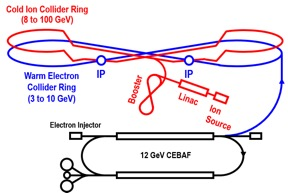
\includegraphics[width=.75\textwidth]{../../img/jleic_schematic2.jpg}
	\caption{Schematic layout of JLEIC}
	\label{fig:jleic1}
\end{figure}

The unique figure-8 shape of the JLEIC collider rings has been chosen to optimally preserve the electron and ion polarizations during acceleration and storage. \cite{Kondratenko:2016eqn}  Each collider ring is partitioned into two arcs and two long straights. The electron and ion collider rings intersect in the horizontal plane at two symmetric points, one in each of the two long straights as shown in Fig. 1; thus, two detectors can be accommodated. The two long straights also support other utility elements of the collider rings including the beam injection and abort systems, RF accelerating and bunching systems, electron cooler, and beam polarimeters.
The JLEIC design provides a high luminosity exceeding $10^{34}$ cm$^{-2}$ s$^{-1}$ at each interaction point. The high luminosity performance is based on high repetition rate, strong focusing at the collision points, and low beam emittances. The figure-8 design produces over 80\% polarization for both the electron and ion beams and allows for efficient polarization control. Table 1 summarizes some of the high-level design parameters for the machine.

\begin{center}
	\begin{tabular}{ l l c c c c } 
		JLEIC Parameters & & \multicolumn{2}{c}{Single-turn ERL Cooler} & \multicolumn{2}{c}{Multi-turn ERL Cooler}\\ 
		& & \multicolumn{2}{c}{PEP-II e-ring} & \multicolumn{2}{c}{New e-ring} \\
		\hline \hline
		& & p & e & p & e\\
		\hline
		Beam energy & GeV & 100 & 5 &100 &5 \\ 
		Collision frequency & MHz& \multicolumn{2}{c}{476} & \multicolumn{2}{c}{476}\\ 
		Particles per bunch & $10^10$ & 0.66 & 3.9& 0.98 & 3.7\\
		Beam current & A & 0.5 & 3 & 0.75 & 2.82\\
		Polarization &  & \textgreater80\% & \textgreater80\% & \textgreater80\% & \textgreater80\%\\
		Bunch length, rms & cm & 1 & 1.2 & 1.2 & 1.2 \\
		Norm. emittance, x/y& $\mu$m & 1/0.5 & 144/72 & 0.5/0.1 & 70/14 \\
		x/y $\beta^*$ & cm &4/2 & 2.6/1.3 & 6/1.2 & 4/0.8\\
		Vert. beam-beam param.& & 0.006 & 0.014 & 0.015 & 0.053\\
		Laslett tune shift & & 0.01 & Small & 0.048 & Small\\
		Detector space, up/down & m & 3.6/7 & 2.4/1.6 & 3.6/7 & 2.4/1.6\\
		Hourglass (HG)reduction & & \multicolumn{2}{c}{0.88} & \multicolumn{2}{c}{0.80}\\
		Lumi./IP, w/ HG, $\mathbf{10^{33}}$ & cm$^{-2}$ s$^{-1}$ & \multicolumn{2}{c}{4.6} & \multicolumn{2}{c}{19.5} \\
		\hline
		%\caption{Parameters and luminosity for a full-acceptance detector.}
		\label{table:parameters}
	\end{tabular}
\end{center}

While thorough background studies must be completed for the specific parameters of the machine, the background issues to be studied in this project are common to any EIC design and the tools and techniques to be developed in this project will be applicable to and allow benchmarking of other EIC designs.

\subsubsection{Full-Acceptance Detector region design}

As illustrated in \ref{fig:detector_concept}, accessing the EIC physics requires reconstruction of a whole event. In particular, one must detect small-angle products including the recoiling target baryon (3D structure of the nucleon), hadrons produced from its breakup (target fragmentation), or all the possible remnants produced when using nuclear targets (including the tagging of spectator protons in polarized deuterium), over a wide range of momenta (and charge-to-mass ratios) with respect to the original ion beam.

From simple kinematics, the reaction products are biased towards small angles around the original ion beam. From machine design and luminosity considerations, it is not desirable to leave a very large detector space free of beam focusing elements to allow the small-angle products to accumulate sufficient transverse separation from the incident beams. The solution is to let the small-angle particles pass through the nearest elements of the machine final-focusing system, which simultaneously perform the function of angle and momentum analyzer for the small angle reaction products. A significant challenge of this approach is that it has to consistently reconcile often contradictory detector and machine optics requirements.

\begin{figure}
	\centering
	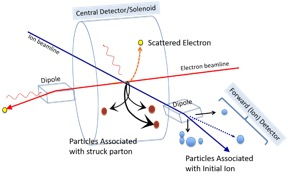
\includegraphics[width=.75\textwidth]{../../img/central_detector.jpg}
	\caption{Detector concept.}
	\label{fig:detector_concept}
\end{figure}

Figure 3 shows a schematic layout of one of the JLEIC interaction regions containing a full-acceptance detector.  \cite{Abeyratne:2012ah} \cite{Abeyratne:2015pma}  \cite{Lin} \cite{Morozov:2012} \cite{Morozov:2014} 
The electron and ion beams cross at a relatively large angle of 50 mrad, which greatly improves the momentum resolution for hadrons detected within a few degrees of the ion beam direction, and provides fast separation of the two beams thus eliminating parasitic bunch collisions and allowing one to move the final focusing elements closer to the interaction point (IP). The electron beam is aligned with the detector axis to avoid generation of synchrotron radiation.


\begin{figure}
\centering
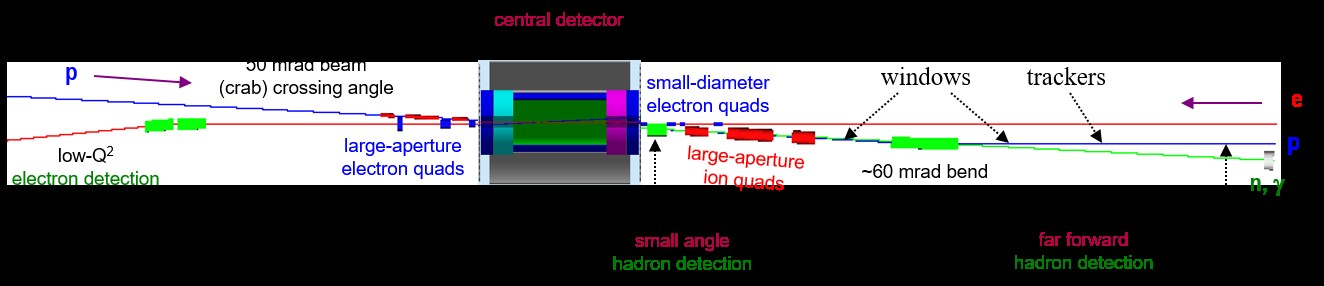
\includegraphics[width=.75\textwidth]{../../img/detector_schematic.jpg}
\caption{Schematic layout of the JLEIC full-acceptance detector region.}
\label{fig:detector_concept}
\end{figure}

The central detector is built around a 4 m long solenoid extending 2.4 m on the outgoing ion side and 1.6 m on the opposite side. The solenoid field is adjustable independently of the beam energies in order to optimize the detection for various processes. The maximum field is expected to be 3 T. The solenoid is surrounded by 2 m long detector end caps. Electrons scattered at small angles ($<0.5^{\circ}$) are detected in a low-Q2 tagger consisting of large-aperture electron Final Focusing Quadrupoles (FFQ) and a spectrometer dipole with a few meters of instrumented space on either side.

In addition to benefiting from the large crossing angle in the solenoid, charged hadrons with scattering angles below $3^{\circ}-5^{\circ}$ with respect to the ion beam will pass through a large-aperture 2 Tm dipole (Dipole 1) located before the ion FFQs. The dipole is 1.5 m long and is followed by 0.5 m of drift space and detectors. Particles at very small angles ($<0.5^{\circ}$)  will pass through the ion FFQs and then, after a few meters of a drift space, through a 56 mrad dipole (Dipole 2) for momentum analysis. Various detector elements are placed in the space between the final focus and Dipole 2 as well as beyond the dipole to provide complete angular and momentum coverage.

The primary full-acceptance detector has a sufficiently large magnet-free space near the interaction point (IP) for detection of particles down to about 0.5 in front of the final focus blocks. In addition, to allow detection of particles scattered between $0^{\circ}-0.5^{\circ}$, the hadrons and electrons need to pass through the large-aperture final focusing quadrupoles and are detected by the further downstream (up to 37 m) detector components \cite{Abeyratne:2012ah} \cite{Abeyratne:2015pma}  \cite{Lin} \cite{Morozov:2012} \cite{Morozov:2014}. To maximize the detector’s acceptance to the forwarding scattered hadrons and electrons, both the ion and electron beams are focused downstream of the forward final focus so that small beam sizes at the focal points allow one to place the detectors closer to the beam centers. In combination with ~1 m dispersion at those points, this allows detection of particles with small momentum offset $\Delta p/p$. This optics should be optimized to maximize its angular and momentum acceptance and detector resolution. 

The interaction region optics is optimized to meet the above detection requirements as shown in Figure \ref{fig:magnet_optics} (left) and Figure \ref{fig:magnet_optics} (right) for ions and electrons, respectively. In particular, the detector space is made asymmetric by leaving a large 7 m distance from the IP to the first ion FFQ in the downstream ion direction where the reaction products tend to go, while having the upstream ion FFQs placed closer to the IP at 3.5 m to minimize their chromatic contribution. A weak spectrometer dipole is placed in front of the downstream ion FFQs.

The downstream ion and electron final focusing quads are designed with large apertures for forward detection and are followed by spectrometer dipoles. Additionally, as shown in Figure \ref{fig:magnet_optics}, both the ion and electron beams are focused again towards the ends of the element-free spaces downstream of the respective spectrometer dipoles to allow closer placement of the detectors at those locations, which, in combination with the relatively large dispersion values there, enhances the forward detectors’ momentum resolution. The dispersion generated by the spectrometer dipoles is suppressed on the ion side by a specially designed section, which also controls the beam line geometry, while on the electron side the dispersion suppression is done by a simple dipole chicane whose parameters are chosen to avoid a significant impact on the electron equilibrium emittances. The chicane is designed to accommodate a Compton polarimeter and a luminosity monitor \cite{Morozov:2014}. Special attention is paid to sizes and positions of the detector region elements to avoid them interfering with each other and with the detector functionality. 

\begin{figure}
	\centering
	\begin{minipage}{0.45\textwidth}
		\centering
		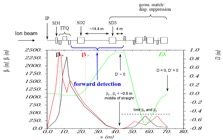
\includegraphics[width=.75\textwidth]{../../img/ion_magnet_optics}
	\end{minipage}\hfill
	\begin{minipage}{0.45\textwidth}
		\centering	
		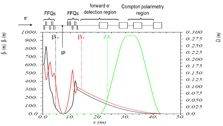
\includegraphics[width=.75\textwidth]{../../img/electron_magnet_optics}	
	\end{minipage}
	\caption{Magnetic optics of the ion (left) and electron (right) detector regions.}
	\label{fig:magnet_optics}
\end{figure}

The full-acceptance detector region has been integrated into the electron and ion collider ring lattices with necessary optical and geometric matching. As shown in Fig. \ref{fig:jleic1}, the detector is placed far from the electron arc exit to minimize the synchrotron radiation background and close to the ion arc exit to minimize the hadronic background due to the ion beam scattering on the residual gas.

Figure 5 shows an expanded view of the detector region layout. The end section of the ion arc upstream of the IP is shaped to produce a 50 mrad horizontal crossing angle between the ion and electron beams while the ion beam line segment downstream of the IP is designed to produce a 1.5 m transverse separation between the ion and electron beams. The same section is used to suppress the dispersion. The electron detector region has no net bend or shift. This makes the collider ring geometry somewhat independent from the detector region design and simplifies its optimization \cite{Lin}.

Due to the strong beam focusing at the IP, the chromatic effect of the FFQs in both the ion and electron collider rings is very significant and requires proper compensation but is manageable. Chromatic compensation is done using properly arranged sextupoles in the rings’ arcs \cite{Nosochkov:2015}.

\begin{figure}
	\centering
	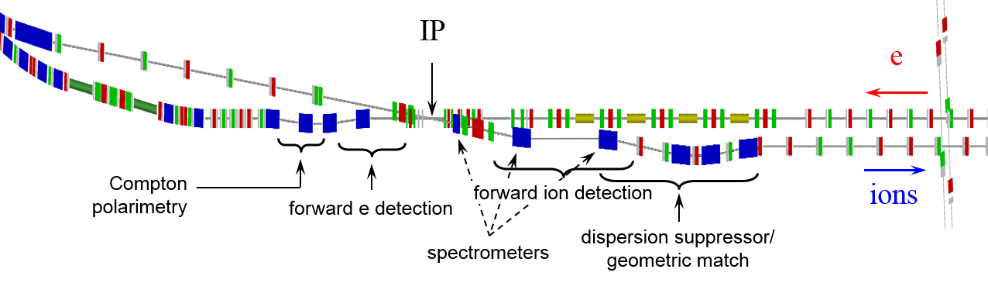
\includegraphics[width=.75\textwidth]{../../img/detector_region_layout}
	\caption{Detector Region Layout}
	\label{fig:detector_region_layout}
\end{figure}

\subsection{Proposed Work}

$\cdot$ Input from Latifa and Kijun\\

We define that background is the event in which experiments are affected by unwanted particles entering from the machine.
Such background can interfer the machine regular operation and even worsly have a potential damage that ends up machine
failure, including Crab cavity failure and asynchronous beam dump.


In general, machine background should be well understood not only in advance of the machine operation but also optimal
design of detectors as well as shielding. The lesson from the HERA II commissioning after the upgrade, very severe
backgrounds were observed, and the machine had to be shut down for several months. While studies of the backgrounds
were performed and solutions to mitigate the backgrounds were installed. Their major source of background comes from
large proton beam-gas interactions and increased synchrotron radiation. Since a proposed Electron-Ion-Collider(EIC)
is similar machine as HERA (electron-proton-collider) although there are many different features, their major background
sources could be same issue.


Recently, LHC had dedicated tests during 2015-2016 to understand machine-induced background through studying in terms of
a loss map for beam-halo, pressure bump for local beam-gas interaction. In particular, it turned out that beam-gas interaction
is the most dominant background by high limunosity experiment analysis results \cite{Bruce:2016}.


The proposed study will focus on estimating machine-induced backgrounds to the detectors, giving crucial information
to all groups designing detector systems on the radiation environment in which the devices will operate. The study
will additionally be applicable for two EIC designs.



In reality, there are crucial questions related to machine-induced background that should be addressed:
\begin{itemize}
\item{1} Can we understand better at what level background become problematic ?
\item{2} What can we demonstrate such background ? How we can evaluate these ?
\item{3} Waht can be done to improve safty for operation ?
\end{itemize}



In simplification, the goals of this proposal is following:
\begin{itemize}
\item{1} Identify the background sources for given baseline design parameters
\item{2} Quantify the background level
\item{3} Suggest or provide possible solution or modification
\end{itemize}

Firt of all, it is very important to identify what is the background source that causes severe problem during beam operation
or detection capability. For example, synchrotron radiation is very critical source for tracking detector near the interaction
point. Hence shielding or controlling this radiation is key to improve the tracking efficiency. Secondly, once we know source
of background, we should evaluate how much background level will be expected for given operational parameters. By doing this
study, it will immediately provide an idea or solution how we can improve or optimize the run configuration or detector design
or shielding.


$\cdot$ Emphasize aspects of common interest bewteen eRHIC and JLEIC. \\


In this proposal, we would like to study various source of machine-induced backgrounds, such as Synchrotron radiation,
 Beam-gas interactions, Beam halo, Beam losses, Neutron flux and Radiation from elastic scattering. Such backgrounds
 are major and common concerns independent of machine. However, they are not always clearly indentified as separated
 effects.  We hence propose a study for any correlation among these sources with respect to accelerator machine and
 detector design through sophisticated Monte Calro simulation based on GEANT4 with various event generators.
Therefore this will be a very important study for both eRHIC and JLEIC to understand and evaluate all these sources
with respect to design parameters and operational configurations.


Detailed simulation studies need to be performed for the relevant background sources.
A subset of sources of background we will study are itemized section.XXX.
Such simulation results will be directly input to improve experimental detector response.




\subsection{Technical Approach}
\subsubsection{Workflow}
this is a placeholder for workflow
\subsubsection{Synchrotron Vacuum}
This is a placeholder for contributions from Marcy and/or Mike regarding synchrotron and vacuum.
\subsubsection{Optimization}
%\input{optimization.tex}
\subsubsection{Validation with HERA}
*not necessarily its own section.
%input{../approach/validation.tex}
\subsection{Collaborative Efforts}
Team organization.
\section{Deliverables}
Several project deliverables will be achieved with the completion of this study.  Specifically:
\begin{itemize}[label=\textbullet]
	
		\litem{} Develop simulation code and CAD model for most current interaction region design, especially with regard to new beam pipe design and variations, which is necessary for all future EIC physics simulations. 
	
		\litem{}Develop and validate new and existing simulation packages to model synchrotron radiation and examine path of radiation, shielding design, collimation schemes, and provide recommendations for layout changes if necessary.
		
		\litem{} Use simulation of synchrotron radiation to quantify and track this background in detectors.  Determine the amount and locations of energy deposited and evaluate any impact to  design.
		
		\litem{} Compare background from synchrotron radiation to the rate of physics events in a study of signal to background. 
		
		\litem{} Perform detailed study of vacuum pressure distribution in and around the IR.  This is necessary to achieve an accurate estimate of beam-gas event rates in the detectors.  Furthermore, this study underlies vacuum pump placement and begins an iterative design process in collaboration with the machine design group, especially with regards to beam pipe design.
		
		\litem{} Implement JLEIC configuration and event generator with existing, benchmarked packages to model beam-gas interactions.
		
		\litem{} Quantify and track background from beam-gas interactions to determine impact on beam and physics measurements.
		
		\litem{} Quantify levels of neutron flux by collaborating with Radiation Control division to model experimental area and determine its impact. 
		
		\litem{} Optimize placement of auxiliary detectors for reducing background: for instance, positioning the high luminosity monitor at ion exit arc to reduce hadronic and synchrotron backgrounds.)
					
		\litem{} Provide feedback to the machine design group in an iterative process to help guide the design optimized for physics.
		
		\litem{} Overall, model and quantify background radiative load as a function of angle to help guide detector technology design choices and optimization of placement.  This will form the basis for not only the background studies but future physics simulations.  
	
	\end{itemize}
\section{Budget}
%\section{Summary}

\section{References}
\bibliography{../../bib/bib}
\bibliographystyle{plain}

%%This is reference numbering guide, to be deleted in final version:
\begin{enumerate}
	\item \cite{Abeyratne:2012ah} Abeyratne:2012ah
	\item \cite{Abeyratne:2015pma} Abeyratne:2015pma
	\item \cite{Aschenauer:2016} Elke's prop
	\item \cite{Bruce:2016} Bruce:2016
	\item \cite{Carter:2016} Carter:2016
	\item \cite{ZEUS:1993} ZEUS
	\item \cite{Furletova:2015pma} Furletova:2015pma
	\item \cite{Holzer:2009} Holzer:2009
	\item \cite{Kondratenko:2016eqn} Kondratenko:2016eqn
	\item \cite{Lin:2013} Lin:2013
	\item \cite{Morozov:2012} Morozov:2012
	\item \cite{Morozov:2014} Morozov:2014
	\item \cite{Morozov:2015} Morozov:2015
	\item \cite{Niebuhr:2009} Niebuhr:2009
	\item \cite{Nosochkov:2015} Nosochkov:2015
	\item \cite{Seidel:2004} Seidel:2004pma(hera)
	\item \cite{Sosa:2016} Sosa:2016
	\item \cite{Ungaro} Ungaro
\end{enumerate}

\appendix
\section{Software Benchmarking by HERA Experience}
To establish the validity of future simulations using current software tools, GEMC~\cite{Ungaro}, Geant4, and the JLEIC initial distribution generator were benchmarked against background rates measured at HERA following the luminosity upgrade.  By replicating HERA conditions, simulations produced background rates that were comparable to those recorded in HERA's C5 detector.  Successfully reproducing these rates validates several software tools for background studies and underscores both the need and readiness to conduct JLEIC background studies at this time.

\subsection{HERA Issues and Lessons}

Following the HERA-II upgrade in 2000 and 2001, high levels of beam-induced background were observed and identified: synchrotron radiation, proton gas scattering, lepton gas scattering, and proton beam halo losses.   In fact, 95\% of background observed following the upgrade came from proton beam-gas interactions where vacuum conditions had deteriorated due to synchrotron radiation.  The background impacted the detectors and necessitated a several month shutdown to perform simulations and remediate the problem.

High levels of synchrotron radiation had been expected after the HERA upgrade, since the luminosity increase was achieved by stronger beam focusing (lower $\beta^*$) and required upgraded focusing magnets, changes to the machine lattice, and a redesigned IR. Unique vacuum chamber geometry, collimators, and masks were installed to handle the expected increase in background.  However, adequately detailed background studies were not conducted ahead of time, and these changes generated significantly more machine-induced background than anticipated.  A several month shutdown was necessary to perform additional simulations and develop mitigation strategies.  Until 2004, HERA-II operations were current-limited due to background.

During the shutdown, the HERA team performed detailed simulations of the dynamic pressure profile and residual beam gas analysis to determine the best mitigation strategies.  Results indicated that vacuum pressure, dominated by hydrogen gas, spiked to $10^{-8}$ mbar in the region spanning $\pm$ 5 m around the IP.   This  was 100 times higher than the nominal pressure of $10^{-10}$ mbar achieved at the location of the vacuum pumps.  Beam particles interacted with the hydrogen gas, producing halo particles which constituted a large portion of the background events reaching the ZEUS detector.  The C5 counter was placed very close to the beam pipe to measure the rate and arrival times of these halo particles.
%%Insert pictures of vacuum and gas analyses

%\begin{figure}
%	\centering
%	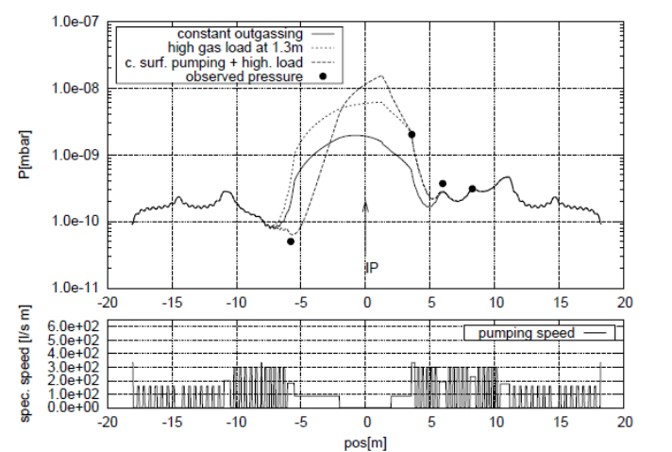
\includegraphics[width=.75	\textwidth]{../../img/hera_badvac_regions.jpg}
%	\caption{HERA-II Vacuum pressure distribution around the IP following upgrade.  Minima correspond to placement of the vacuum pumps.}
%	\label{fig:hera1}
%\end{figure}
%\begin{figure}
%	\centering
%	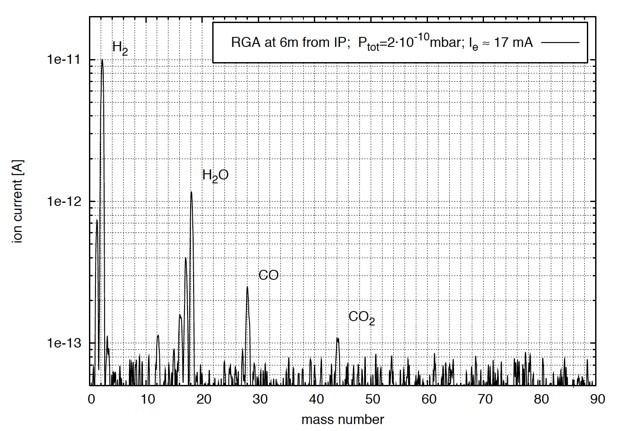
\includegraphics[width=.75\textwidth]{../../img/hera_badvac_comp.jpg}	
%	\caption {HERA-II Composition of beampipe gas 6 m from IP. }
%	\label{fig:hera2}
%\end{figure}

\begin{figure}[!hbt]
	\centering
	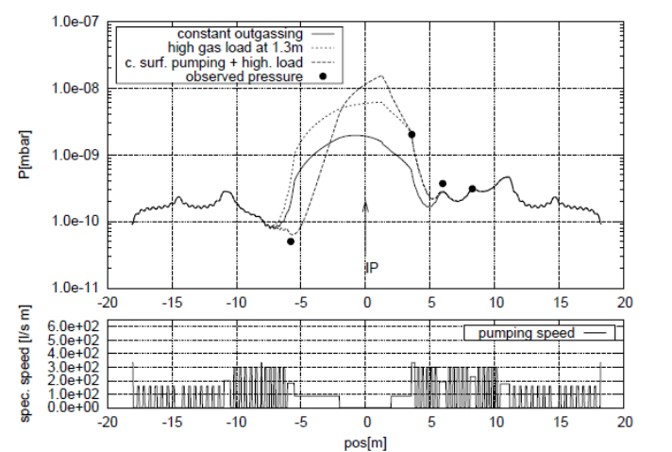
\includegraphics[width=.48\textwidth]{../../img/hera_badvac_regions.jpg}
	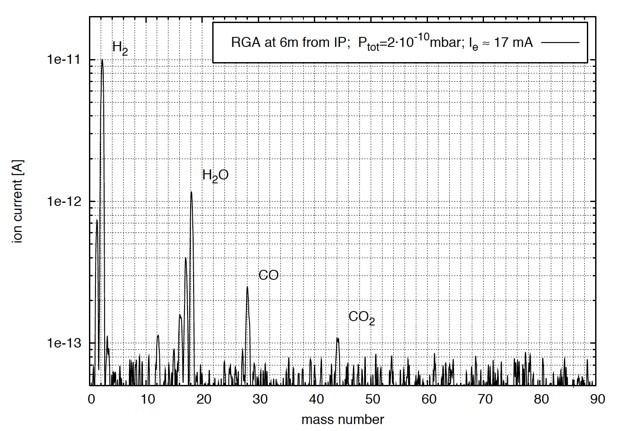
\includegraphics[width=.48\textwidth]{../../img/hera_badvac_comp.jpg}	
	\caption {\textbf{Left}: HERA-II Vacuum pressure distribution around the IP following upgrade.  Minima correspond to placement of the vacuum pumps. \textbf{Right}: Composition of beampipe gas at 6 m from IP. }
	\label{fig:hera2}
\end{figure}



\begin{figure}[!hbt]
	\centering
	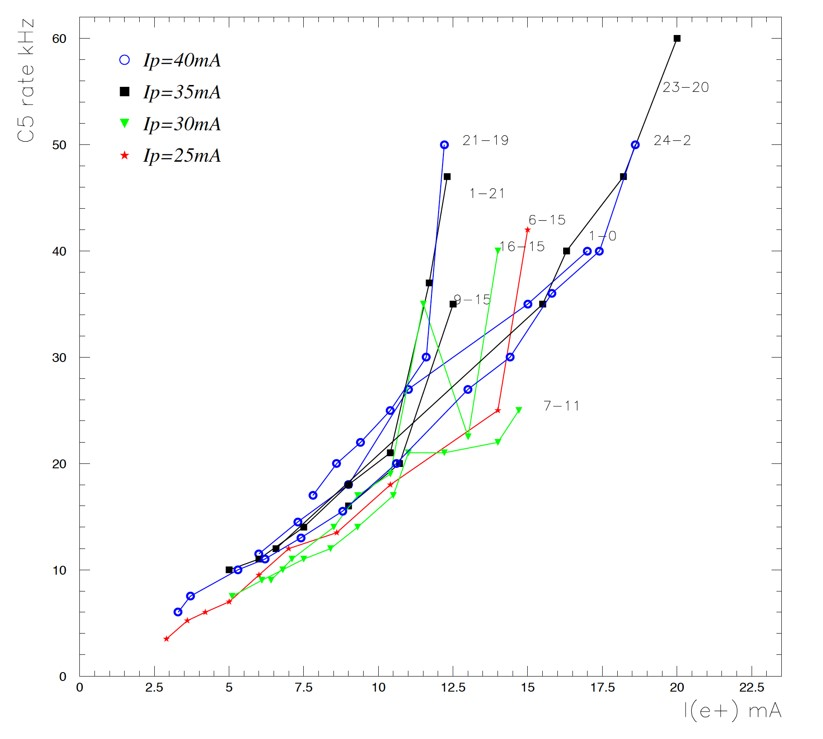
\includegraphics[width=.65\textwidth]{../../img/hera_c5_rate.jpg}
	\caption{C5 rate as a function of HERA \textit{e} beam current for different \textit{p} beam current.  Numeric tags indicate the date and hour of the beginning of \textit{ep} injection for July 2002.}
	\label{fig:hera3}
\end{figure}

\subsection{Detector Geometry}

The C5 detector was a silicon tungsten sandwich counter comprised of eight scintillator tiles mounted in pairs above and below the beampipe, orthogonal to the z axis.  The arrangement of the 3 mm thick tiles created an octagon with an outer profile of 20 cm by 20 cm, as shown in Figure \ref{fig:hera5}.  The detector was positioned 1240 mm upstream from the IP around the cylindrical aluminum beampipe of radius 19 mm.  
%insert pictures of C5 Detector placement

\subsection{Detector Rates}
The primary uses of the C5 detector were:
\begin{itemize}
	\item to detect the presence of halo particles in order to reduce background event rates in ZEUS.
	\item to provide rate and arrival time measurements for monitoring and controlling HERA beam conditions.
	\item to calculate the $Z$ vertex position.
\end{itemize}
Figure \ref{fig:hera3} shows the C5 rates as a function of HERA electron beam current for several proton beam currents.  Although the rates in the C5 varied as a function of current, they provide a range by which to base the benchmarking study.  Figure \ref{fig:hera3} indicates that the rate in the C5 detector was approximately 10 kHz for I$_{p}$ = 40 mA, for I$_{e+}$ between 2 mA and 7 mA. 
%insert c5 rates

\subsection{Approach}

In order to benchmark simulation tools against the observed background rates, a virtual detector was modeled after the C5 detector and positioned at the same location relative to the IP.  A beam pipe with the same specifications as the original was filled with a hydrogen target of density proportional to the vacuum quality of the corresponding region at HERA.  

Key parameters were either matched to the HERA case, scaled, or shown to exert little influence over the event rate.  These are summarized below:

\begin{center}
	\begin{tabular}{ l l l }[!hbt]
		& HERA & Simulated \\ 
		\hline \hline
		Gate Time & 96 ns & 100 ns \\ 
		$p$ bunch length & 100 mm & n/a \\ 
		$I_p$ & 100 mA & 100 mA\\
		$E_p$ (GeV)& 920 & 900 $\pm$ 1 \\
		$N$/bunch & $10^{11}$ & $10^{11}$\\
		$N$ Events & n/a & $\approx 10^6$\\
		vacuum near IP& $10^{-8}$ mbar  & 1 g/cm$^3$ H \\
		Vacuum else& $10^{-10}$ mbar & 0.01 g/cm$^3$ H\\
		Gas & 95\% H & 100\% H\\
		\hline
	\end{tabular}
\end{center}


To replicate the C5 detector, a two-disc scintillator detector was built in GEMC and placed 1240 mm upstream from the IP.  Like the actual C5 detector, the virtual detector was comprised of discs 3 mm thick, separated by 20 mm.  The inner and outer radii also matched the original: $R_{in} = 3.801/2$ cm and $R_{out} = 20.0/2$ cm.  The detector was assigned "flux" sensitivity, so that different tracks record different hits independent of the time window. 
\begin{figure}[!htb]
	\centering
	\begin{minipage}{0.45\textwidth}
		\centering
		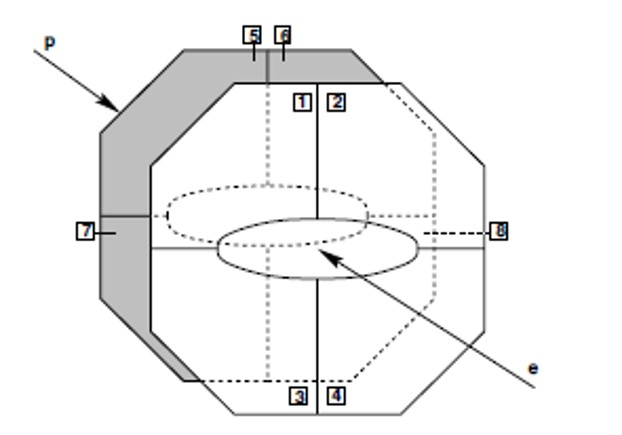
\includegraphics[width=.8\textwidth]{../../img/hera_c5.jpg}
		\caption {Schematic of the actual C5 Time of Flight Detector  }
		\label{fig:hera5}
	\end{minipage}\hfill
	\begin{minipage}{0.45\textwidth}
		\centering	\includegraphics[width=.75\textwidth]{../../img/C5_gemc}	
		\caption {Virtual C5 detector rendered in GEMC.}
		\label{fig:hera6}
	\end{minipage}
\end{figure}

HERA's beampipe from 2002 was replicated by modeling a simple cylindrical beam pipe out of 0.5mm thick aluminum with inner radius 19mm.  It was filled with hydrogen gas of density proportional to  $10^{-8}$ mbar $\pm$5 m around IP and $10^{-10}$ mbar everywhere else.

GEMC's native beam distribution generator was initialized directly before the higher pressure region and fired approximately $10^6$ protons toward the IP.  Both 100 and 900 GeV particles were simulated, with a momentum spread of $\pm$ 1 GeV, 0.2 mrad spread in $\phi$ and $2\pi$ rad spread in $\theta$.  All particles hitting the detector, both charged and neutral, were recorded and their information stored in an EVIO file.  Data was analyzed in ROOT after file conversion and making a cut along the $z$ axis in the location of the detector.  The number of neutral particles recorded in the detector was then subtracted from the total, and counts were normalized to exactly $10^6$ events.  This number, along with previously stated assumptions and scale factors, was used to calculate the rate of particles seen in the virtual C5 and compared to HERA-II data.

The basic HERA configuration was simulated: i.e., a 900 GeV proton beam was fired from the center of the beam pipe in front of the higher density gas region and the detector hits were recorded.  Two Geant4 physics models were compared and the results are noted below.  Additionally, simulations were performed to compare the results of lower beam energy, external beam distribution generator with JLEIC parameters, varying degraded vacuum region length, varying degraded vacuum region density, and varying beam pipe composition.

\begin{figure}[!hbt]
	\centering
	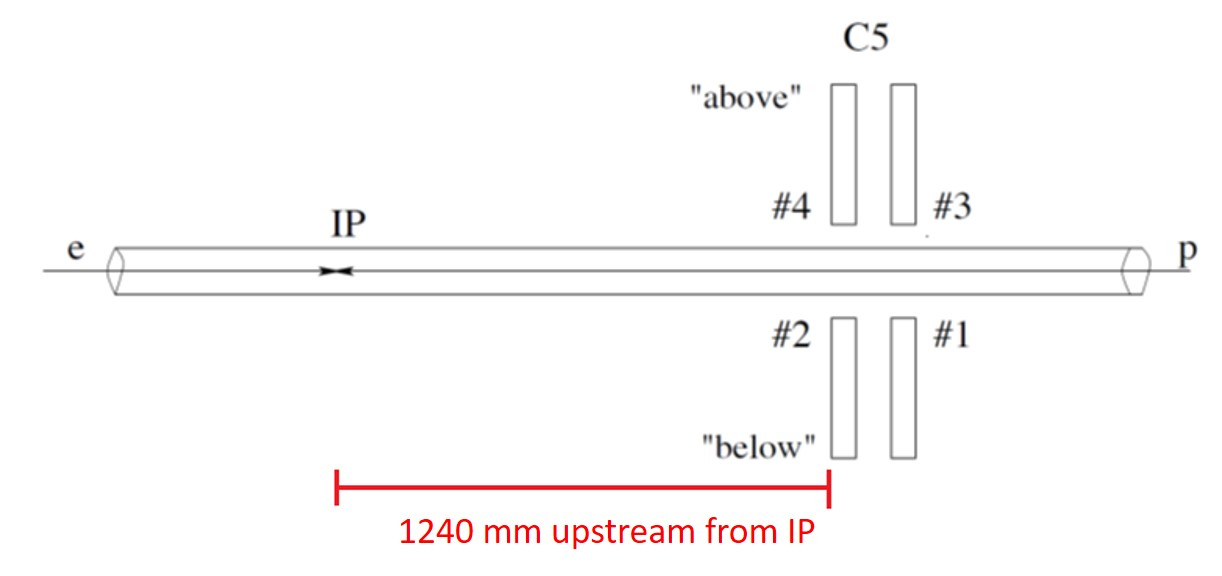
\includegraphics[width=.75\textwidth]{../../img/c5_placement.jpg}
	\caption{C5 detector placement along HERA beamline.}
	\label{fig:hera4}
\end{figure}

\subsection{Analysis and Results}
The rate of particles in the virtual C5 detector was calculated by $I = qE\cdot N/t$.  With HERA parameters, the virtual C5 detector measured approximately 33kHz for charged particle events, which compares favorably to HERA data.  

Additional simulations verified the relationship between vacuum density and length of degraded vacuum region.  Increasing the density of the hydrogen gas produced higher event rates, as expected.  Similarly, increasing the length of the degraded vacuum region produced higher event rates than the baseline HERA configuration.  The results of these comparisons are reproduced in Figure \ref{fig:hera5} and \ref{fig:hera6}, with the HERA configuration highlighted.

\begin{figure}[!hbt]
	\centering
	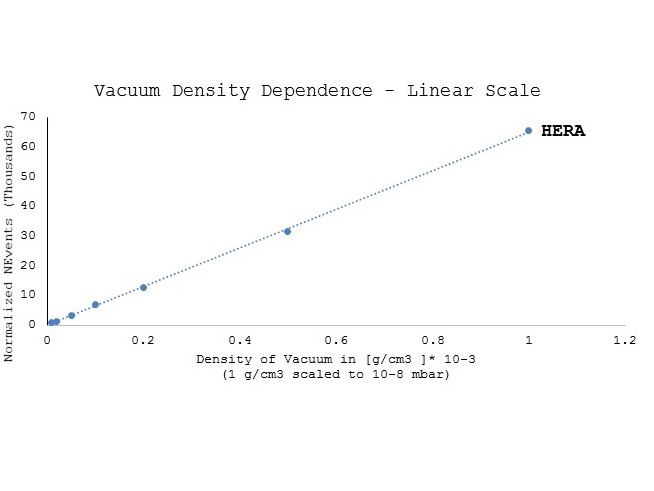
\includegraphics[width=.75\textwidth]{../../img/density_dep_lin_crop.jpg}
	\caption {C5 rate as a function of vacuum density, with an arbitrary linear fit.}
	\label{fig:hera5}
\end{figure}	

\begin{figure}[!hbt]
	\centering	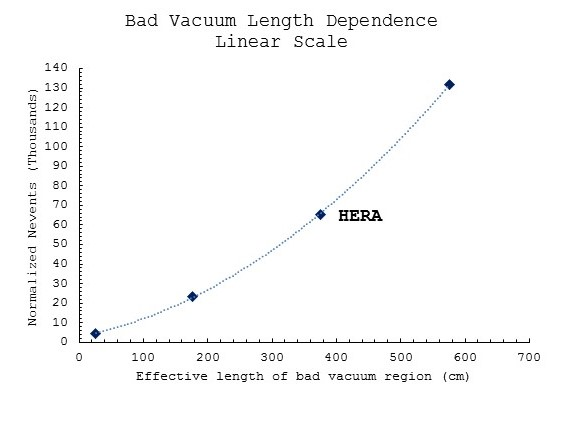
\includegraphics[width=.75\textwidth]{../../img/length_dep_poly_crop.jpg}	
	\caption {C5 rate as a function of degraded vacuum region length, with an arbitrary polynomial fit.}
	\label{fig:hera6}
\end{figure}



Simulations  performed to compare beam energy at 100 GeV and 900 GeV did not produce noteworthy differences in background rates.  Additional studies comparing the GEANT4 physics models found event rates to be approximately 25\% higher using the FRITIOF precompound model (FTFP) versus the Quark-Gluon String Precompound model (QGSP).  Beam pipe composition was also compared, and aluminum beam pipes were found to produce 25\% more background than a beryllium/aluminum mix.


%show: occupancy plot?


\subsection{Conclusion}
The benchmarking study has confirmed that using HERA parameters, the GEMC software produces data in agreement with the experimental results from HERA.  Additionally, the initial distribution generator, which accurately models JLEIC beam parameters, indicates similarly high levels of proton beam-gas background for HERA vacuum conditions.  This validates future results produced with these tools and reinforces both the need and readiness to undertake further studies of the beam gas interactions generated in the EIC.  

To build upon these studies, it is necessary to implement the IR beam pipe design in GEMC and CAD in order to 

\begin{itemize}
	\item Determine the influence of EIC IR geometry on proton beam-gas background using EIC initial  bunch distributions.
	\item Validate the assertion that $10^{-9}$ mbar vacuum pressure provides tolerable vacuum conditions and begin to develop possible pumping schemes.
	\item Validate the synchrotron radiation event generator in GEANT4/GEMC.
	\item Determine figure-of-merit for synchrotron radiation due to electron beam-gas interactions.
	\item Evaluate the effectiveness of a small chicane along the upstream electron beamline for minimizing the beamline synchrotron radiation contribution.
\end{itemize}

Such measures are within the scope of this proposal.












%\begin{figure}
%	\centering
%	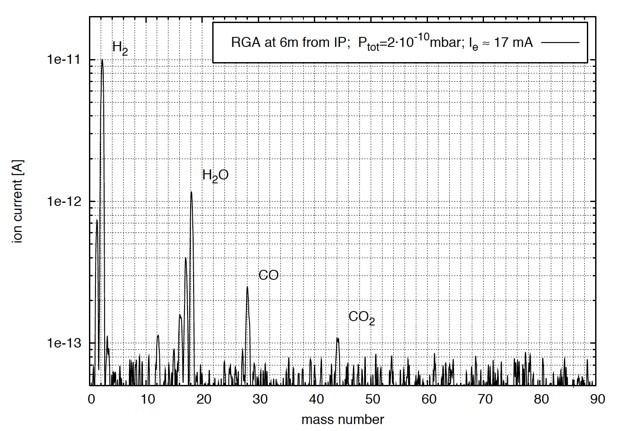
\includegraphics[width=.75\textwidth]{../../img/hera_badvac_comp.jpg}
%	\caption{HERA-II Vacuum pressure distribution in the IR.  The vacuum in the region $\pm$ 5m around the IP deteriorated to $10^{-8}$ mbar, compared to $10^{-10}$ mbar achieved at the pump locations.}
%	\label{fig:hera1}
%\end{figure}

%\begin{figure}
%	\centering
%	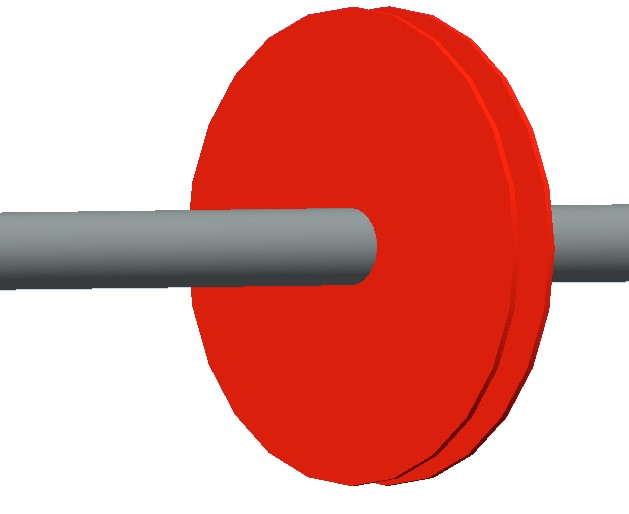
\includegraphics[width=.75\textwidth]{../../img/c5_gemc.jpg}
%	\caption{HERA-II Vacuum pressure distribution in the IR.  The vacuum in the region $\pm$ 5m around the IP deteriorated to $10^{-8}$ mbar, compared to $10^{-10}$ mbar achieved at the pump locations.}
%	\label{fig:hera1}
%\end{figure}

%\begin{figure}
%	\centering
%	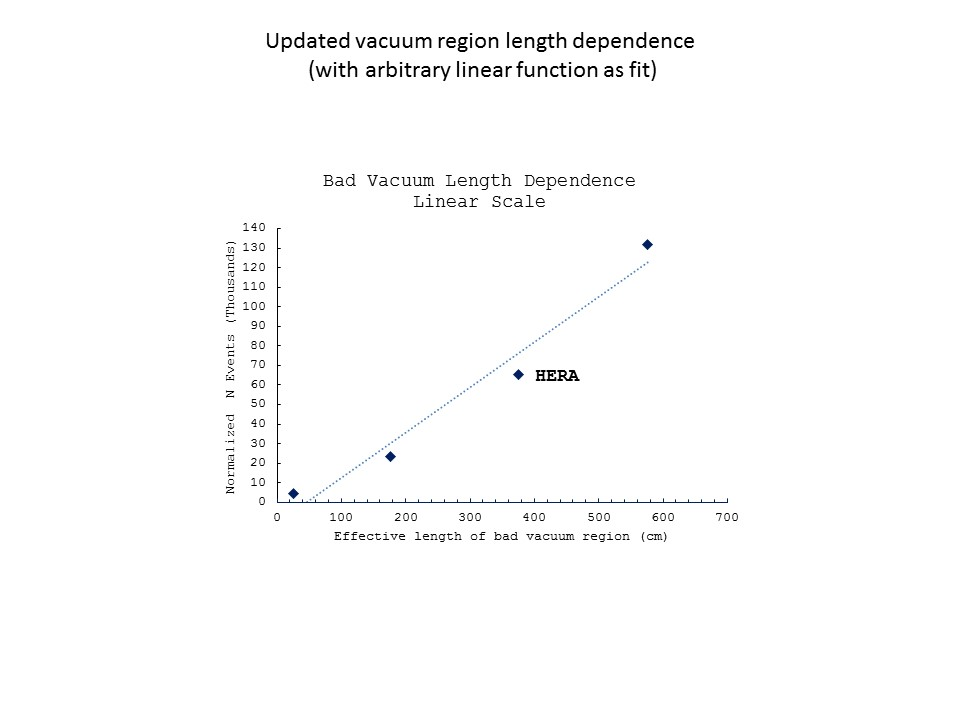
\includegraphics[width=.75\textwidth]{../../img/length_dep_linear.JPG}
%	\caption{HERA-II Vacuum pressure distribution in the IR.  The vacuum in the region $\pm$ 5m around the IP deteriorated to $10^{-8}$ mbar, compared to $10^{-10}$ mbar achieved at the pump locations.}
%	\label{fig:hera1}
%\end{figure}

%\begin{figure}
%	\centering
%	\includegraphics[width=.75\textwidth]{../../img/ length_dep_log.JPG}
%	\caption{HERA-II Vacuum pressure distribution in the IR.  The vacuum in the region $\pm$ 5m around the IP deteriorated to $10^{-8}$ mbar, compared to $10^{-10}$ mbar achieved at the pump locations.}
%	\label{fig:hera1}
%\end{figure}

%\begin{figure}
%	\centering
%	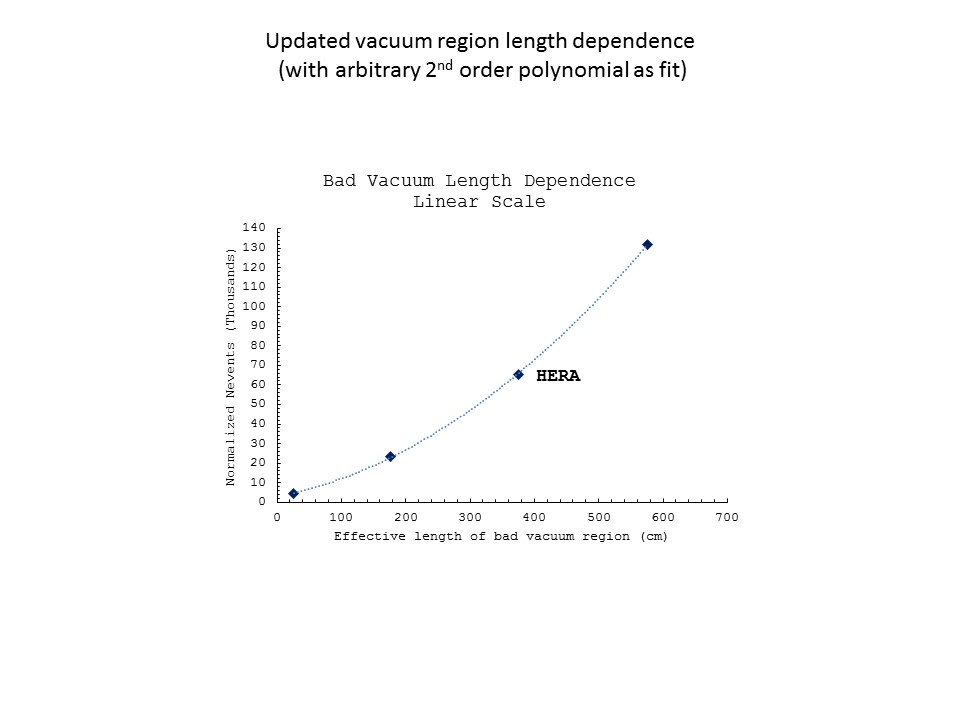
\includegraphics[width=.75\textwidth]{../../img/length_dep_poly.JPG}
%	\caption{HERA-II Vacuum pressure distribution in the IR.  The vacuum in the region $\pm$ 5m around the IP deteriorated to $10^{-8}$ mbar, compared to $10^{-10}$ mbar achieved at the pump locations.}
%	\label{fig:hera1}
%\end{figure}

%\begin{figure}
%	\centering
%	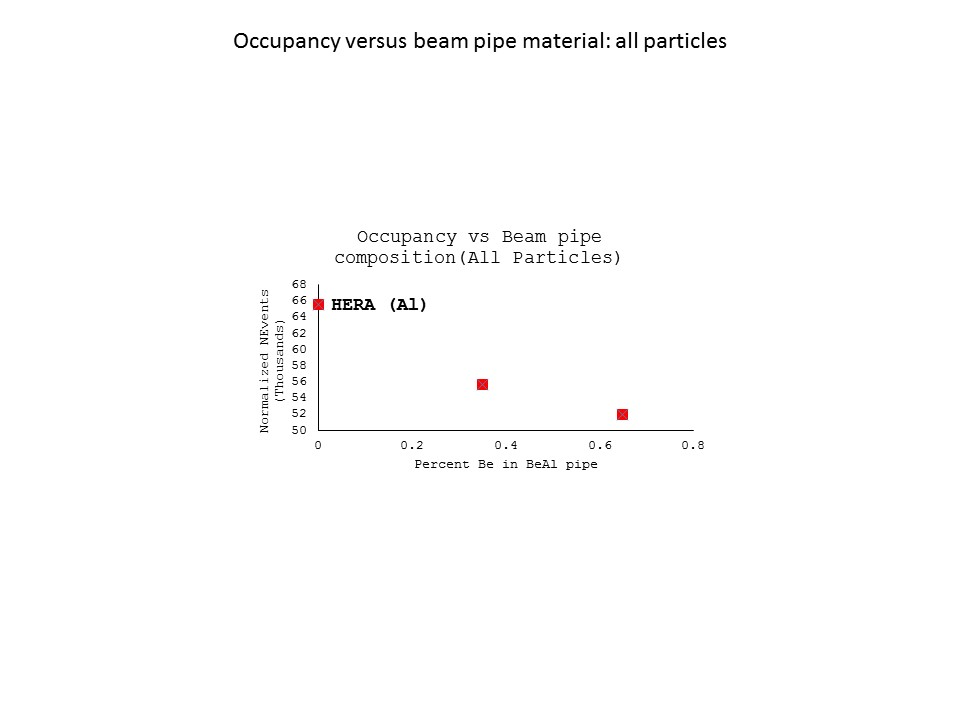
\includegraphics[width=.75\textwidth]{../../img/pipe_comp_all.JPG}
%	\caption{HERA-II Vacuum pressure distribution in the IR.  The vacuum in the region $\pm$ 5m around the IP deteriorated to $10^{-8}$ mbar, compared to $10^{-10}$ mbar achieved at the pump locations.}
%	\label{fig:hera1}
%\end{figure}

%\begin{figure}
%	\centering
%	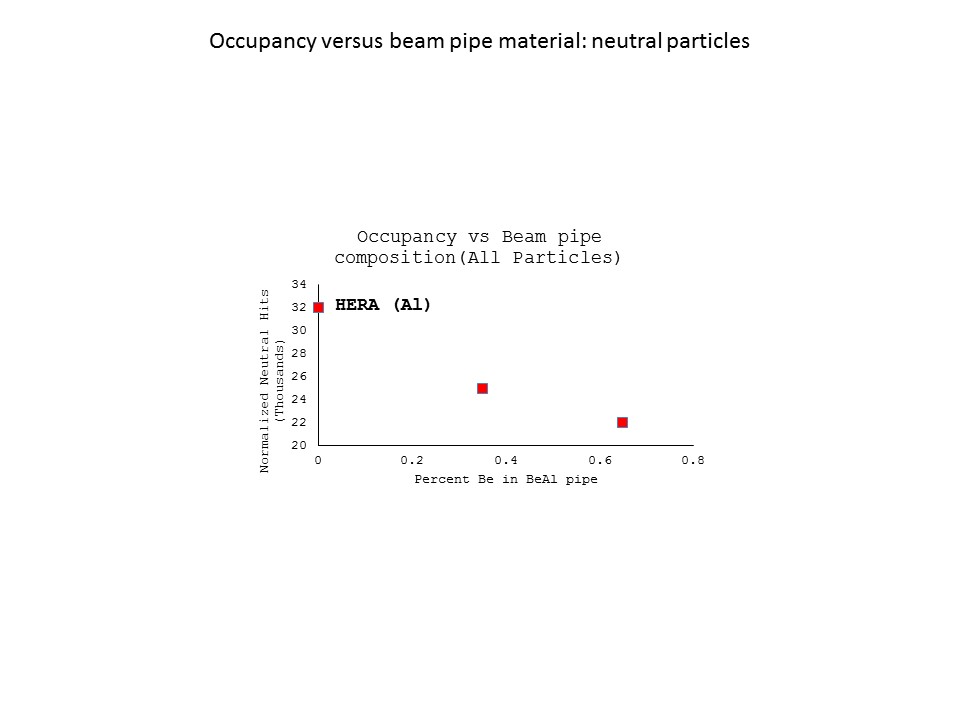
\includegraphics[width=.75\textwidth]{../../img/pipe_comp_neutral.JPG}
%	\caption{HERA-II Vacuum pressure distribution in the IR.  The vacuum in the region $\pm$ 5m around the IP deteriorated to $10^{-8}$ mbar, compared to $10^{-10}$ mbar achieved at the pump locations.}
%	\label{fig:hera1}
%\end{figure}

%Simple table
%\begin{center}
%	\begin{tabular}{ |c|c|c| } 
%		\hline
%		cell1 & cell2 & cell3 \\ 
%		cell4 & cell5 & cell6 \\ 
%		cell7 & cell8 & cell9 \\ 
%		\hline
%	\end{tabular}
%\end{center}



\end{document}

